\documentclass{article} % For LaTeX2e
\usepackage{nips12submit_e,times}
%\documentstyle[nips12submit_09,times,art10]{article} % For LaTeX 2.09

\def\argmax{\operatornamewithlimits{arg\max}}

\title{Exact Symbolic Dynamic Programming for Continuous POMDPs}


\author{
%Zahra Zamani \\
%ANU & NICTA\\
%Canberra, Australia \\
%\texttt{zahra.zamani@anu.edu.au} \\
%\And
%Coauthor \\
%Affiliation \\
%Address \\
%\texttt{email} \\
%\AND
%Coauthor \\
%Affiliation \\
%Address \\
%\texttt{email} \\
%\And
%Coauthor \\
%Affiliation \\
%Address \\
%\texttt{email} \\
%\And
%Coauthor \\
%Affiliation \\
%Address \\
%\texttt{email} \\
%(if needed)\\
}

% The \author macro works with any number of authors. There are two commands
% used to separate the names and addresses of multiple authors: \And and \AND.
%
% Using \And between authors leaves it to \LaTeX{} to determine where to break
% the lines. Using \AND forces a linebreak at that point. So, if \LaTeX{}
% puts 3 of 4 authors names on the first line, and the last on the second
% line, try using \AND instead of \And before the third author name.

\newcommand{\fix}{\marginpar{FIX}}
\newcommand{\new}{\marginpar{NEW}}

%\nipsfinalcopy % Uncomment for camera-ready version

\begin{document}

\maketitle

\begin{abstract}
Decision-theoretic planning searches for the optimal sequence of actions for a given uncertain environment. Partially Observable MDPs (POMDP) can model such environments where the underlying state is not be fully observable. %While discrete models of the environment is often used for planning, continuous models are naturally closer to the real-world. 
While previous work have provided solutions for discrete states and/or observations, here we define the first exact solution to both continuous state and observations. The symbolic dynamic programming approach in this paper avoids enumerating the state and observation space providing solutions for general multi-variate discrete and continuous POMDPs. Our main contribution is that for a fixed set of reachable belief states and a fixed set of actions, only a \textit{finite} partitioning of the continuous observation space is required for optimality. 
Using function representation of Affine algebraic decision diagrams (XADDs) and symbolic case operators we derive the automatic partitioning for piecewise linear dynamics %such as the reward, transition and observation function. 
We demonstrate empirical results on an operation research domain to show the \textit{first exact solution} to continuous state and observation POMDPs.  
%to use continuous states with discrete observations and extending it to continuous observations by defining relevant observation partitions %associated with each state partition. %This allows us to perform the Bellman backup operation efficiently. 
%We address the problems in POMDP continuous planning and solutions to solve them symbolically. %To compactly represent the exact value functions Affine algebraic decision diagrams are used. 
\end{abstract}

\section{Introduction}
% Write intro here
In many complex systems complete information of the state is not available due to noisy or poor sensors and readings of them. Partially observable Markov Decision Processes (POMDPs)\cite{POMDPfirst} can be used for planning under such uncertainty in such problems. The solution to a POMDP is to find an answer to the fully-observable belief-MDP, whose states are probability distributions over the state space of the original POMDP \cite{kaebling}
Real-world resources and sensor inputs are often naturally modelled using continuous variables. 
Unfortunately most POMDP techniques can not be applied to such settings without assuming prior knowledge about the problem domain. Most methods use some approximation to discretize the continuous state, observation or action space which increases computational complexity \cite{Thrun99h}. The optimal value function of belief-MDPs is piecewiselinear and convex in these discrete cases \cite{sondik71} but has also been proven in the setting of only continuous states. \cite{PerseusObs}

Exact solutions to a multi-variate continuous state and observation setting has not been approached for the curse of dimensionality problem. In assuming a continuous observation setting, the agent must search for all possible observations that are read from the environment. This can quickly become infeasible even for small problem sizes. 

In this paper we provide an exact solution to a subset of POMDPs with continuous states and observations. Our symbolic dynamic programming (SDP) approach assumes discrete noise and piecewise linear dynamics and functions. We formulize our problems using a Discrete and Continuous POMDP (DC-POMDP) model and apply our SDP algorithm. The main problem that rises in any problem modeled using DC-POMDP is the definition of different observation partitions and their probability. We apply symbolic solutions such as integration and maximization to provide an optimal closed-form solution to our problem domains. 
As an example we consider the following power plant example which has mainly been solved in the literature using discrete sets of states and observations~\cite{steam2}. We use the example throughout the paper to help better understand the definitions. 

\textbf{Example} \textsc{(Power Plant)}
\emph{The steam generation system of a power plant aims to provide hot steam to the steam turbine which in turn produces electricity. Feed-water is exposed to heat in the tubes leading to the water tank . Evaporating the water is performed under specific pressure and temperature inside the attached water tubes. 
Mixing water and steam pressures makes reading tank levels and temperatures very hard and uncertain. For this reason, the process is modeled using POMDP in the literature. The temperature $t_s \in \mathbb{R}$ is modelled as a continuous state variable. Noisy observation of the temperature $t_o \in \mathbb{R}$ is used to help decide the optimal action to either open or close the pressure valve $a \in \{open,close\}$.}

We need to extend the basic SDP framework from \cite{sanner_uai11} by adding continuous observations to the model. The solution to a closed-form value function is similar to the algorithm from \cite{monahan82} apart from the fact that no explicit observation is defined in the continuous case. We redefine the value-iteration algorithm using case representations that are implemented using Extended Algebric decision diagrams (XADD) and provide an efficient automatic way to partition the entire observation space into piecewise linear functions where each partition has a relative probability. We use the univariate \textsc{Power Plant} example to define the main operations and algorithms and also provide empirical results for a multi-variate version of the problem. 

\section{DC-POMDP Model} 
%%%% no need to define DC-MDP
We assume familiarity with MDPs and introduce Discrete and Continuous Partially Observable MDPs as an extension to Discrete and Continuous State MDPs ~\cite{sanner_uai11}. A Discrete and Continuous partially observable MDP (DC-POMDP) is a tuple $\langle
\mathcal{S},\mathcal{A},\mathcal{O},\mathcal{T},\mathcal{R},\mathcal{Z},\gamma,h \rangle$. 
States are represented by vectors of $(\vec{d_s},\vec{x_s}) = ( d_{s_1},\ldots,d_{s_n},x_{s_1},\ldots,x_{s_m} )$ where each $d_{s_i} \in \{ 0,1 \}$ ($1 \leq i \leq n$) is a discrete boolean and each $x_{s_j} \in  \mathbb{R}$ ($1 \leq j \leq m$) is a continuous variable. Actions are presented by a finite set of actions $\{ a_1, \ldots, a_p \}$. We define discrete and continuous observations by the vector $(\vec{d_o},\vec{x_o}) = ( d_{o_1},\ldots,d_{o_n},x_{o_1},\ldots,x_{o_m} )$ where each $d_{o_i} \in \{ 0,1 \}$ ($1 \leq i \leq n$) is boolean and each $x_{o_j} \in \mathcal{R}$ ($1 \leq j \leq m$) is a continuous variable. 

Three functions are required for modeling DC-POMDPs: (1) $\mathcal{T}: \mathcal{S} \times \mathcal{A} \times \mathcal{S} \rightarrow  [ 0, 1 ]$ a Markovian transition model defined as the probability of the next state given the action and previous state %$P(\vec{d}',\vec{x}'|\cdots,a)$
; (2)  $\mathcal{R}:\mathcal{S}\times\mathcal{A} \rightarrow \mathbb{R}$ a reward function which returns the immediate reward of taking an action in some state and (3) an observation function defined as $\mathcal{Z} : \mathcal{S} \times \mathcal{A} \times \mathcal{O} \rightarrow [ 0, 1 ]$  which gives the probability of an observation given the outcome of a state after executing an action.  A discount factor $\gamma, \; 0 \leq \gamma \leq 1$ is included in the model to account for future rewards in higher horizons.

%%%% forms of transition, observation and reward function
To define the transition and observation function, we use the fact that the state variables of this POMDP can be factored into a Dynamic Bayesian Network (DBN). Not allowing synchronic arcs between the discrete and continuous variables defines their joint transition or observation to be independent: 
%{\footnotesize
%\begin{equation}
%P(\vec{d_s}',\vec{x_s}'|\vec{d_s},\vec{x_s},a) = 
%\prod_{i=1}^n P(d_{s_i}'|\vec{d_s},\vec{x_s},a) \prod_{j=1}^m P(x_{s_j}'|\vec{d_s},\vec{d_s}',\vec{x_s},a). \nonumber 
%\end{equation}}
%The joint observation function can also be defined considering the direct correspondence between the state and observation variables:
{\footnotesize
\begin{equation}
P(\vec{d_o},\vec{x_o}|\vec{d_s},\vec{x_s},a) = 
\prod_{i=1}^n P(d_{o_i}|d_{s_i},a) \prod_{j=1}^m P(x_{o_j}|x_{s_j},a). \nonumber 
\end{equation}}
\emph{Binary} variables are represented using conditional probability functions (CPF) in the form of $P(d_i'|\vec{d},\vec{x},a)$. \emph{Continuous} variables
$P(x_j'|\vec{d},\vec{d'},\vec{x},a)$ are represented by \emph{piecewise
linear equations} (PLEs) that are first-order Markov and deterministic, i.e. the probabilities are encoded using the Dirac $\delta[\cdot]$ function. The reward function $R(\vec{d},\vec{x},a)$ is set to be any general piecewise linear  function that could facilitate pruning for space efficiency.% via bilinear solvers. 
%%%%%%%%%%%%%%%%%%%%%%%%%%%%%%%%%%%%%%%%%%%%%%%%%%%%%%%%%%%%%%%%%%%%%%%%
% Figure 1 - policy tree
\begin{figure}[t!]
%\vspace{-1mm}
\begin{center}
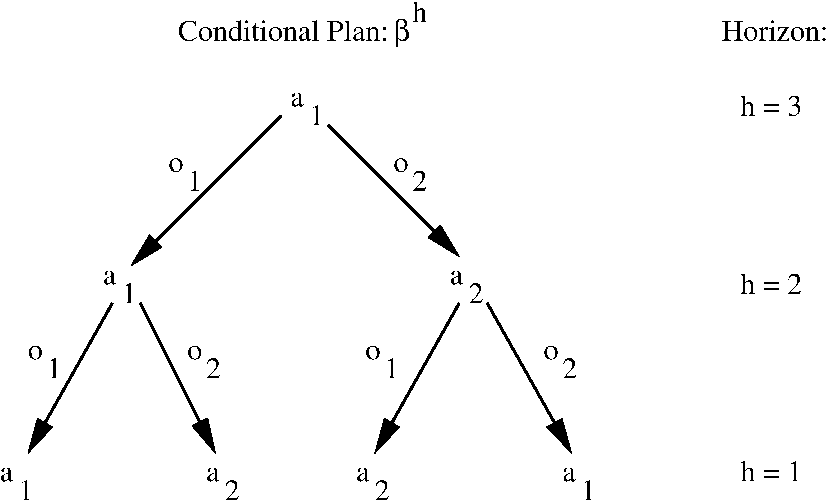
\includegraphics[width=0.4\textwidth]{pics/cond_plan2.pdf}
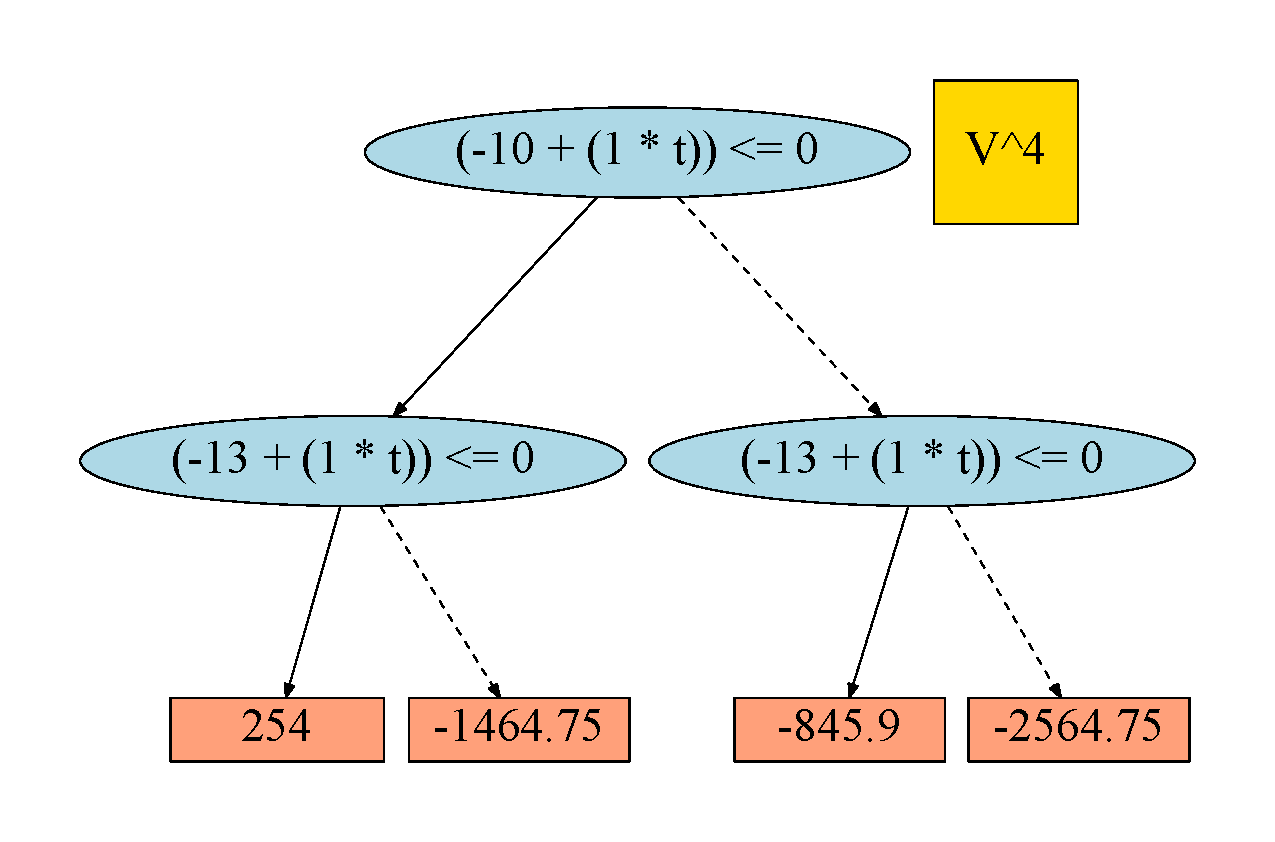
\includegraphics[width=0.45\textwidth]{pics/b1-4.pdf}
\end{center}
\vspace{-2mm}
\caption{\footnotesize Left: Example conditional plan $\beta^h$ for discrete observations. Right: The optimal value function for \textsc{Power Plant}
as a decision diagram: 
the \emph{true} branch is solid, the \emph{false}
branch is dashed.}
\label{fig:cond_plan}
\vspace{-1mm}
\end{figure}
%%%%%%%%%%%%%%%%%%%%%%%%%%%%%%%%%%%%%%%%%%%%%%%%%%%%%%%%%%%%%%%%%%%%%%%%
%%%%%%%%%%%%%%%%%%%%%%%%%%%%%%%%%%%%%%%%%%%%%%%%%%%%%%%%%%%%%%%%%%%%%%%%%%%
%\begin{figure}[t]
%\begin{center}
%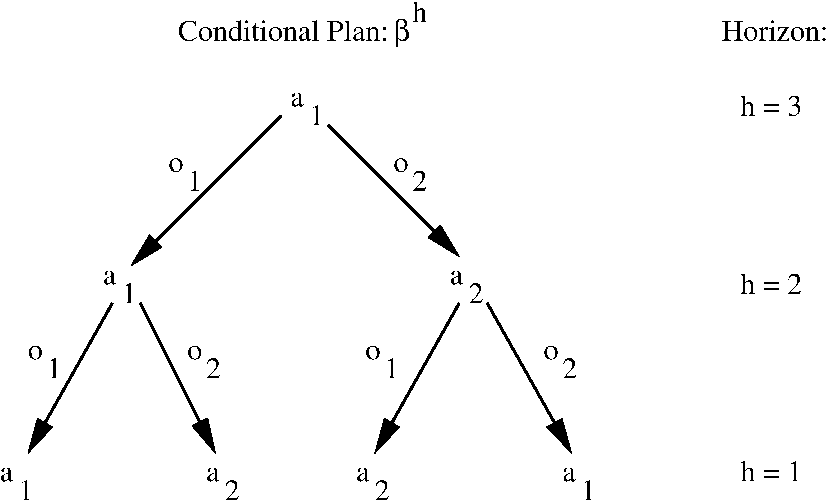
\includegraphics[width=0.4\textwidth]{pics/cond_plan2.pdf}
%\end{center}
%\vspace{-3mm}
%\caption{%\footnotesize 
%The optimal value function for \textsc{Power Plant}
%as a decision diagram: 
%the \emph{true} branch is solid, the \emph{false}
%branch is dashed.} 
%\end{figure}
%%%%%%%%%%%%%%%%%%%%%%%%%%%%%%%%%%%%%%%%%%%%%%%%%%%%%%%%%%%%%%%%%%%%%%%%%%%
For the \textsc{Power Plant} example, the transition and reward functions are defined as below:
% For the transition probability, we use the Dirac function to model the deterministic equations. We can also define stochasticity in the transition model using boolean random variables that are sampled stochastically.  The reward function can be any linear function of the state or action. Going above a threshold temperature (e.g. $T=10$) will cause an explosion in the plant when trying to close the valve which results in the negative reward of $-1000$. Staying below this temperature is safe and will produce electricity an gain the reward of $100$. The reward of an open valve is $-1$.
{\footnotesize
\begin{align}
P(t_s'|\vec{t_s},a)= \delta\left[ t_s' - 
\begin{cases}
 (a=open) &: t_s - 5 \\ 
(a \neq open) &: t_s + 7 \\
\end{cases}
\right]\nonumber
\hspace{5mm}
R(t_s,a) = 
\begin{cases}
 (a=open) &: -1 \\
(a \neq open)\wedge (t_s>T) &: -1000 \\
(a \neq open)\wedge \neg(t_s>T) &: 100 \\
\end{cases}\nonumber
\end{align}
}
%contribution? 
This example will try to maximize its reward using observations on the temperature. The observations received before closing the plant to a safe temperature are therefore critical.  For the observation model we begin with a discrete model for two observations $t_{o_1},t_{o_2}$ such as the following for the $open$ action:  
{\footnotesize
\begin{align}
P(t_{o_1}|t_s',open) = 
\begin{cases}
 \delta\left[ t_s <= 15 \right] &: 0.9 \\
 \delta\left[ \neg (t_s <= 15)\right] &: 0.1 \\
\end{cases}\nonumber
\hspace{5mm}
P(t_{o_2}|t_s',open) = 
\begin{cases}
 \delta\left[ t_s <= 15 \right] &: 0.1 \\
 \delta\left[ \neg (t_s <= 15)\right] &: 0.9 \\
\end{cases}\nonumber
\end{align}
}
%\\
%P(t_{o_1}|t_s',close) = 
%\begin{cases}
% \delta\left[ t_s <= 15 \right] &: 0.1 \\
% \delta\left[ \neg (t_s <= 15)\right] &: 0.8 \\
%\end{cases}\nonumber
%,
%P(t_{o_2}|t_s',close) = 
%\begin{cases}
% \delta\left[ t_s <= 15 \right] &: 0.9 \\
% \delta\left[ \neg (t_s <= 15)\right] &: 0.2 \\
%\end{cases} \nonumber
%\end{align}
After defining the solution to the discrete observation with a continuous state DC-POMDP, we can extend this to consider continuous observations using a continuous uniform noise distribution which is more realistic in many domains. %For a certain interval, the probability is a fixed number, while it is zero elsewhere. The integral of the uniform distribution should sum to one. 
{\footnotesize
\begin{align}
P(t_o|t_s',open) = 
\begin{cases}
 (t_o>t_s-5) \wedge (t_o<t_s+5) &: 0.1 \\
 \neg((t_o>t_s-5) \wedge (t_o<t_s+5)) &: 0 \\
\end{cases}\nonumber
\end{align}
}
Next we define the general solution to solving DC-POMDPs. 


\section{DC-POMDP solution}
The DC-POMDP will choose actions in order to compute an optimal plan over time. This plan is the policy $\pi$ of the agent  depending on the history of actions and observations over a Markovian state. In the partially observable case where there is uncertainty on the states, the policy is a function over a continuous set of probability distributions over $|\mathcal{S}|$ known as the belief state $b = P(x_s,d_s)$.

At any of the horizon steps, a DC-POMDP policy $\pi(b)$ is defined as the iterative plan on executing an action and observing all probable outcomes of the set of observations from the $(h-1)$-step. The belief state is updated after this according to the Bayes rule: $\sum_{d_s}\int_{x_s} b(xd_s)T(xd'_s,xd_s,a)Z(xd'_s,xd_o,a)$. \footnote{For simiplicity we use ($xd_s = x_s,d_s$) and ($xd_o=x_o,d_o$)}
The optimal policy is defined over the belief state as the sum of the expected discounted rewards over horizon $h$ starting with belief $b_0$.
{\footnotesize
\begin{equation}
V^h_{\Pi^*}(\vec{b}) = E_{\pi^*} \left[ \sum_{h=0}^{H} \gamma^t \cdot r_h \Big| \vec{b}_0 = \vec{b} \right]\nonumber
\end{equation}
}
Solving the value function for the optimal policy is performed using Dynamic programming algorithms such as value iteration. 
%The decision at each time step is to pick an action based on past actions and observations. 
The possible set of conditional plans $\beta^h$ correspond to a decision tree. Figure 1 left, shows the decision tree for the simple case of three horizons with discrete observations. It represents a conditional plan consisting of an action and two possible observation strategies. For continuous observations, conditional plans are decision trees with infinitely many branches. In our solution we show that instead of a policy tree with infinite branches, we can create partitions based on relevant observation values, resulting in a policy tree similar to that of figure 1. %From here on we assume this finite set of observation partitioning as $\mathcal{O}$.
%%%%%%%%%%%%%%%%%%%%%%%%%%%%%%%%%%%%%%%%%%%%%%%%%%%%%%%%%%%%%%%%%%%%%%%%
\incmargin{.5em}
\linesnumbered
\begin{algorithm}[t!]
\vspace{-.5mm}
\dontprintsemicolon
\SetKwFunction{backup}{Backup}
\SetKwFunction{genObs}{GenRelObs}
\SetKwFunction{prune}{Prune}
\SetKwFunction{remapWithPrimes}{Prime}
\Begin
{
   $V^0:=0, h:=0$\;
   \While{$h < H$}
   {
       $h:=h+1, \Gamma^h :=\emptyset$\;
       \ForEach {$a \in A$}
       {
			$\Gamma_{a}^h :=\emptyset$ \;       		
       		\If {$ContObs =true$}
       			{$P(xd_{o_i}|xd_{s_i}) \,:=\,$ \genObs{$\Gamma^{h-1},a,b_i$}\;}
       		 \ForEach {$xd_{o_i} \in \textsc{O}^{h-1}$}
       		 {
				\ForEach {$\alpha_j^{h-1} \in \Gamma^{h-1}$}
       			{
   	 		  		$\alpha_j^{h'}=$ \remapWithPrimes{$\alpha_j^{h}$} \;
   	 		  		\emph{// $\forall$ $d_i \to d_i'$ and $\forall x_i \to x_i'$} \; 
   	 		    	$\Gamma_{a,xd_{o_i},j}^h \,:=\, P(xd_{o_i}|xd_{s_i}) \otimes$ \backup{$\alpha_j^{h'},a$}\;
       	      	}
       	      	$\Gamma_{a,xd_o}^h\,:=\,\textrm{\large $\boxplus$} \Gamma_{a,xd_{o_i}}^h$\;
       	     }
           $\Gamma_a^{h} \,:=\,R_a \oplus \gamma \cdot \Gamma_{a,xd_o}^h$\;
            $\Gamma^{h} \,:=\, \Gamma^{h} \cup \Gamma_a^{h}$\;
        }  
        	%monahan's pruning first generates all vectors, then prunes
              $\Gamma^h \,:=\, $\prune{$\Gamma^h$} \;
              $V^h \,:=\, \mathrm{max}_{\alpha_j \in \Gamma^h} b_i \cdot \alpha_j$\;
              $\pi^{*,h} \,:=\, \argmax_{a} \, \Gamma_a^{h}$\;

       \If{$V^h = V^{h-1}$}
           {break $\,$ \emph{// Terminate if early convergence}\;}
   }
     \Return{$(V^h,\pi^{*,h})$} \;
}
\caption{\footnotesize \texttt{VI}(DC-POMDP, $H$,$ContObs$, $b_i$) $\longrightarrow$ $(V^h,\pi^{*,h})$ \label{alg:vi}}
\vspace{-1mm}
\end{algorithm}
\decmargin{.5em}
%%%%%%%%%%%%%%%%%%%%%%%%%%%%%%%%%%%%%%%%%%%%%%%%%%%%%%%%%%%%%%%%%
For discrete observations and discrete states the number of belief states is infinite, but the optimal value function for $h$ is proven to be a piecewise linear and convex function of the belief state \cite{smallwoodSondik}. The optimal value function is the maximum value over a finite set of alpha vectors  $\alpha^h_i$:%that define the hyperplanes:
{\footnotesize
\begin{equation}
V^h_{\Pi^*}(\vec{b}) = \max_{\alpha^h_i \in \Gamma^h} \alpha^h_i \cdot \vec{b}
\end{equation}
}
where the belief states $\vec{b}$ and each $\alpha^h_i \in \Gamma^h$ are of dimension $|\mathcal{S}|$. 

Point-based dynamic programming backups compute the optimal value function given a belief state $b$. The best conditional plan for the given belief, corresponds to an $\alpha$-vector which is computed using point-based backups: 
{\footnotesize
\begin{align*}
\alpha^{h+1}(b) = R(b) + \gamma \int_{xd_o} P(xd_o|a,b)\alpha^{h+1}(b)\nonumber
\end{align*}
}
where $P(xd_o|a,b) = \int_{xd_s}\int_{xd'_s}b(s)P(xd'_s|xd_s,a)P(xd_o|xd'_s,a)$.

Calculating all possible ways of building the value function independent of a certain belief state can also define the optimal value function. To derive the $\Gamma$-set of all possible $\alpha$-vectors for each horizon, we use the value iteration algorithm from ~\cite{monahan82}. Initializing  $\alpha^0_1 = \vec{0}$ and $\Gamma^0 = \{ \alpha^0_1 \}$, $\Gamma^h$ is obtained from $\Gamma^{h-1}$ using the backup operation defined in (2):\footnote{The $\textrm{\large $\boxplus$}$ of sets is defined as 
$\textrm{\large $\boxplus$}_{j \in \{ 1,\ldots, n \} } S_j = S_1 \textrm{\large $\boxplus$} \cdots \textrm{\large $\boxplus$} S_n$ where the pairwise cross-sum $P 
\textrm{\large $\boxplus$} Q = \{ \vec{p} + \vec{q} | \vec{p} \in P, \vec{q} \in Q \}$.}
{\footnotesize
\begin{align}
V^{h+1}(b) &= \max_a \left( b \cdot r_a + 
\gamma \sum_o \max_{\langle g^h_{a,o,j} \rangle_j}  b \cdot g^h_{a,o,j} \right) \\
\Gamma^{h}_a   &= r_a + \gamma \textrm{\large $\boxplus$}_{o \in \mathcal{O}} \left\{ g^h_{a,o,j}(\cdot) \right\}_j ;  \forall \alpha^{h-1}_{j} \in \Gamma^{h-1}  \\
\Gamma^h  &= \bigcup_a \Gamma^h_a 
\end{align}
}
where $r_a = r(x_s,d_s,a)$ and  
$g^h_{a,o,j} =  \int_{x_{s'}} \sum_{d_{s'}} p(xd_o|xd'_s,a)p(xd'_s|xd_s,a) \alpha^h_j(xd'_s)$
%Each action-dependent $\Gamma$ sums over the possible set of $g^h_{a,o,j}(\cdot)$ given an observation model to derive discrete observations $xd_o$ and for all $\alpha^{h-1}_{j} \in \Gamma^{h-1} $. The value $g^h_{a,o,j}(\cdot)$ is computed by summing over all states given the probability functions and previous $\alpha$-vectors.  
Lines 9--16 of the \textsc{VI} algorithm show the above in a general algorithm used for both discrete and continuous observations. 
For all $\alpha$-vectors in the current $\Gamma$-set first an LP-solver is used to prune any inconsistency in the branches of this vector in line 17. A pairwise dominance test is performed where for all $j,k$: $\alpha_j(\vec{s}) \geq \alpha_k(\vec{s})$
The result of this pairwise test is a dominant $\alpha$-vector which is added to the set of $\Gamma^h$. 
%Here the cross-sum operation takes the set of $\alpha$ -vectors for each observation and produces a sum over vectors that depends on the number of previous iteration vectors. 

Note that the $\alpha$-vector set grows exponentially in the number of observations, i.e., $|\Gamma^{h}| = |\mathcal{A}||\Gamma^{h-1}|^{|\mathcal{O}|}$ during the cross-sum operation. For this reason even for a small number of discrete observations, tractable solutions may be hard to define. Here we do not restrict our observations to discrete ones, but extend it to a fully continuous approach where lines 7--8 will be executed to generate relevant observation partitions based on a belief state $b_i$. We use the number of  observation partitions $|\mathcal{O}|$ as the branching factor in the policy tree. We present the symbolic approach required to partition this continuous space. 

\section{Symbolic Dynamic Programming} 
Dynamic programming provides exact solutions to POMDP problems for small domains. As the domain grows, fully enumerating the state, action and observation space leads to intractable solutions even for low horizons. Avoiding this enumeration often requires approximating the solutions. We claim an exact solution using symbolic dynamic programming. The SDP solution for fully observable domains has been presented in \cite{sanner_uai11} %using piecewise constant functions
Our symbolic algorithm deals with continuous observations and states by generating the relevant observation partition at every time step and performing the backup operation using $\alpha$-vectors. We define the requirements to implement the value iteration algorithm for DC-POMDP. 

\subsection{Case Representation and Extended ADDs}
% operations, max, restrict, substitute
%overview + example plant
The \textsc{Power Plant} example represented all functions using the case structure which can be generally defined as:
{\footnotesize 
\begin{align}
f = 
\begin{cases}
  \phi_1: & f_1 \\ 
 \vdots&\vdots\\ 
  \phi_k: & f_k \\ 
\end{cases} \nonumber
\end{align}
}
Where $\phi_i$ are disjoint logical formulae defined over the state $(\vec{d},\vec{x})$ with logical ($\land,\lor,\neg$) combinations of boolean variables and inequalities ($\geq,>,\leq,<$) over continuous variables.  
The $f_i$ are function definitions either linear or quadratic in the continuous parameters. 

For \emph{unary operations} such as scalar multiplication $c\cdot f$ (for some constant $c \in \mathbb{R}$) or negation $-f$ on case statements is simply to apply the operation on each case partition $f_i$ ($1 \leq i \leq k$). 
A \emph{binary operation} on two case statements, takes the cross-product of the logical partitions of each case statement and performs the corresponding operation on the resulting paired partitions.  The cross-sum $\oplus$ of two cases is defined as the following:
{\footnotesize 
\begin{center}
\begin{tabular}{r c c c l}
&
\hspace{-6mm} 
  $\begin{cases}
    \phi_1: & f_1 \\ 
    \phi_2: & f_2 \\ 
  \end{cases}$
$\oplus$
&
\hspace{-4mm}
  $\begin{cases}
    \psi_1: & g_1 \\ 
    \psi_2: & g_2 \\ 
  \end{cases}$
&
\hspace{-2mm} 
$ = $
&
\hspace{-2mm}
  $\begin{cases}
  \phi_1 \wedge \psi_1: & f_1 + g_1 \\ 
  \phi_1 \wedge \psi_2: & f_1 + g_2 \\ 
  \phi_2 \wedge \psi_1: & f_2 + g_1 \\ 
  \phi_2 \wedge \psi_2: & f_2 + g_2 \\ 
  \end{cases}$
\end{tabular}
\end{center}
}
Likewise $\ominus$ and $\otimes$ are defined by subtracting or multiplying partition values.  Inconsistent partitions can be discarded when they are irrelevant to the function value.
The next three operations are required in defining the value iteration algorithm. A \emph{symbolic case maximization} is defined as below:
\vspace{-4mm}
{\footnotesize
\begin{center}
\begin{tabular}{r c c c l}
&
\hspace{-7mm} $\mathrm{max} \Bigg(
  \begin{cases}
    \phi_1: \hspace{-2mm} & \hspace{-2mm} f_1 \\ 
    \phi_2: \hspace{-2mm} & \hspace{-2mm} f_2 \\ 
  \end{cases}$
$,$
&
\hspace{-4mm}
  $\begin{cases}
    \psi_1: \hspace{-2mm} & \hspace{-2mm} g_1 \\ 
    \psi_2: \hspace{-2mm} & \hspace{-2mm} g_2 \\ 
  \end{cases} \Bigg)$
&
\hspace{-4mm} 
$ = $
&
\hspace{-4mm}
  $\begin{cases}
  \phi_1 \wedge \psi_1 \wedge f_1 > g_1    : & \hspace{-2mm} f_1 \\ 
  \phi_1 \wedge \psi_1 \wedge f_1 \leq g_1 : & \hspace{-2mm} g_1 \\ 
  \phi_1 \wedge \psi_2 \wedge f_1 > g_2    : & \hspace{-2mm}f_1 \\ 
  \phi_1 \wedge \psi_2 \wedge f_1 \leq g_2 : & \hspace{-2mm} g_2 \\ 
  \vdots & \vdots
%  \phi_2 \wedge \psi_1 \wedge f_2 > g_1    : & \hspace{-2mm} f_2 \\ 
%  \phi_2 \wedge \psi_1 \wedge f_2 \leq g_1 : & \hspace{-2mm} g_1 \\ 
%  \phi_2 \wedge \psi_2 \wedge f_2 > g_2    : & \hspace{-2mm} f_2 \\ 
%  \phi_2 \wedge \psi_2 \wedge f_2 \leq g_2 : & \hspace{-2mm} g_2 \\ 
  \end{cases}$
\end{tabular}
\end{center}
}
\emph{Restriction} takes a function $f$ to restrict only in cases
that satisfy some formula $\phi$, which we write as $f|_{\phi}$.  
This can be done by simply appending $\phi$ to each case partition
as the left side shows:
{\footnotesize
\begin{center}
\begin{tabular}{r c c l}
%&
%\hspace{-6mm} 
%  $f = \begin{cases}
%    \phi_1: & f_1 \\ 
%   \vdots&\vdots\\ 
%    \phi_k: & f_k \\ 
%  \end{cases}$
%&
&
\hspace{0mm}
  $f|_{\phi} = \begin{cases}
    \phi_1 \land \phi : & f_1 \\ 
   \vdots&\vdots\\ 
    \phi_k \land \phi : & f_k \\ 
  \end{cases}$
&
\hspace{15mm}
$\int_{x_j'} P(x_j'|\cdots) V'^{h} dx_j' = \begin{cases}
    \phi_1: & V'^{h} \{ x_j' = f_1 \} \\ 
   \vdots&\vdots\\ 
    \phi_k: & V'^{h} \{ x_j' = f_k \}  \\ 
  \end{cases}$
  \end{tabular}
\end{center}
}
\emph{Symbolic substitution} simply takes a set $\sigma$ of variables and their substitutions, where
the LHS of the substitution operator $/$ represents the substitution variable and the
RHS of the $/$ represents the expression that should be substituted in its place.
Hence to perform a continuous regression on a more general
representation, we obtain the right side of the above. 

%xadd representation
The data structure of \emph{extended ADD} (XADD)~\cite{sanner_uai11} is used to support
case statements and the required operations.  Here we use continuous SDP for both states and observations in DC-POMDPs. The value functions and $\alpha$-vectors partition into states of equal value, both of which can be represented using XADDs. For increasing efficiency linear constraint feasibility checkers such as LP solvers allow pruning unreachable paths in the XADD. The right picture in Figure 1 is an example of an XADD representation. 

%%%%%%%%%%%%%%%%%%%%%%%%%%%%%%%%%%%%%%%%%%%%%%%%%%%%%%%%%%%%%%%%%
%\incmargin{.5em}
%\linesnumbered
%\begin{algorithm}[t!]
%\vspace{-.5mm}
%\dontprintsemicolon
%\Begin{
%	\emph{any function f has $i$ partitions like $\phi_i:f_i$}\;	
%	\emph{compute UB and LB from $\phi_i$ using constraints on $var$}\;
%    $I=$ \emph{ any $var$-independent $\phi_i$} \;
%    $F = $ \emph{differentiate $f_i$}\;
%    $F = I \otimes [F(UB) - F(LB)]$\;
%    \Return{$F$} \;
%}
%\caption{\footnotesize \texttt{VE}($var,f$) $\longrightarrow$ $F$ }
%\vspace{-1mm}
%\end{algorithm}
%\decmargin{.5em}
%%%%%%%%%%%%%%%%%%%%%%%%%%%%%%%%%%%%%%%%%%%%%%%%%%%%%%%%%%%%%%%%%
\subsection{PBVI for DC State and Discrete Observations} 

For discrete and continuous states and discrete observations, we use the symbolic version of Monahan's algorithm as the DC-POMDP solution. The same approach is required for continuous observations only based on point-based dynamic programming backups.

Given an initial set of beliefs, we can compute the relevant observation partitions explained in the next section and then continue in a similar fashion of having discrete observations. %To visualize we explain of the value iteration algorithm as defined in \texttt{VI} for DC-POMDPs. Each step of the algorithm is explained using the \textsc{Power plant} example for the first three horizons. 
Note that if the input to this algorithm is continuous observations $ContObs=true$ then line 8 finds the relevant observation partitions, else discrete observations are assumed and their probabilities are given in the problem specifications. Also a belief is given as the input and often several beliefs are required to cover the belief space and thus the algorithm is executed for each one of $b_i \in \mathbb{B}$.

For each iteration, the $\alpha$-vector set are case functions that can be primed (line 11--12). 
%For $h=0$, $V^0$ is given in line 2.  For $h=1$ we choose an action, for example $close$ to start with. The $\alpha$-vector set from $h=0$ is empty so line 7--8 of generating the relevant observation partitions is empty. Also priming the vectors and obtaining the product of relevant observations and the backup is an empty set. In line 15 the reward $R(s,close)$ is added to obtain $\alpha^1_{1,close}$ as defined by (8). The same operation is repeated for the $open$ action where $R(s,open)=-1$. Line 16 defines the final $\Gamma$-set: 
%$\Gamma^1 = \{ \alpha^1_{1,open}, \alpha^1_{1,close} \}$.
The \texttt{Backup} algorithm in line 13 takes the primed version of the variables and performs regression on the $\alpha$-vectors. 
\emph{Boolean restriction} is defined where $f|_{b=v}$ restricts a boolean variable $b$ occurring in $f$ to values $v \in \{ 0,1 \}$. This can be done by simply appending $b=v$ to each case partition (logical $\wedge$ of $b=v$ and the logical first-order formulas of $f$). 

\emph{Continuous regression} $\int f(x_{s_j}') \otimes P(x_{s_j}'|\cdots) dx_{s_j}'$ has the form $\delta[x_{s_j}' - h(\vec{z})]$ for the probability over the next state, where $h(\vec{z})$ is a case statement and $\vec{z}$ does not contain
$x_{s_j}'$.  A symbolic substitution is defined for this integration such that any occurrence of $x_{s_j}'$ in $f(x_{s_j}')$ is substituted with $h(\vec{z})$: 
$\int f(x_{s_j}') \otimes \delta[x_{s_j}' - h(\vec{z})] dx_{s_j}' = f(x'_j) \{ x_{s_j}' / h(\vec{z}) \}$

%For $h=2$, for each of the discrete actions, first we generate the probability of the relevant set of observations in the \texttt{GenRelObs} algorithm. This has been done for the $close$ action in the next section and we use the results here. 
%\begin{align}
%P(z_k)=
%\begin{cases}
% (2<t_o<6) &: 0.2 \\
%(-4<t_o<2) &: 0.6\\
%(-8<t_o<-4) &:0.1999
%\end{cases} 
%\nonumber
%\end{align}
%Next for each of the relevant partitions and both $\alpha$-vectors of the previous $\Gamma$ set lines 9--16 are executed. Line 11 will substitute prime values for all state variables. 
Line 13 produces the backup $\alpha$-vector and multiplies it by the weight derived from the relevant observation partition in the continuous case or observation probabilities in the problem description. 
%For each observation, two vectors are formed for each corresponding $\alpha$-vector. For example line 13 for the observation partitions above and $\alpha_1^1,\alpha_2^1$ is defined as:
%\begin{align*}
%\Gamma_{close,z_1,1}^2= 
%\begin{cases} 
%(t_s'>15) &: -600 \\ 
%\neg(t_s'>15) &: 60 \\
%\end{cases}
%\hspace{15mm} 
%\Gamma_{close,z_1,2}^2= \top &:-0.6
%\\
%\Gamma_{close,z_2,1}^2= 
%\begin{cases}
%(t_s'>15) &: -199.999 \\ 
%\neg(t_s'>15) &: 19.999 
%\end{cases}
%\hspace{12mm} 
%\Gamma_{close,z_2,2}^2= \top &:-0.1999
%\\
%\Gamma_{close,z_3,1}^2= 
%\begin{cases}
%(t_s'>15) &: -200 \\ 
%\neg(t_s'>15) &: 20 
%\end{cases}
%\hspace{15mm} 
%\Gamma_{close,z_3,2}^2= \top &:-0.2
%\end{align*}
Line 14 takes the cross-sum of the two sets which takes every possible combination of observations according to the $\alpha$-vectors. 
%\begin{align*}
%\Gamma_{close,1}^2 &= 
%\begin{cases} 
%(t_s'>15) &: -800.2 \\ 
%\neg(t_s'>15) &: 79.8 \\
%\end{cases}
%\hspace{10mm} 
%\Gamma_{close,2}^2= 
%\begin{cases} 
%(t_s'>15) &: -1000 \\ 
%\neg(t_s'>15) &: 100 \\
%\end{cases}
%\\
%\Gamma_{close,3}^2&= 
%\begin{cases} 
%(t_s'>15) &: -800.2 \\ 
%\neg(t_s'>15) &: 79.8 \\
%\end{cases}
%\hspace{10mm}
%\Gamma_{close,4}^2= 
%\begin{cases} 
%(t_s'>15) &: -600.4 \\ 
%\neg(t_s'>15) &: 59.6 \\
%\end{cases}
%\\
%\Gamma_{close,5}^2&= 
%\begin{cases} 
%(t_s'>15) &: -400.5999 \\ 
%\neg(t_s'>15) &: 39.3999 \\
%\end{cases}
%\hspace{5mm} 
%\Gamma_{close,6}^2= 
%\begin{cases} 
%(t_s'>15) &: -200.7999 \\ 
%\neg(t_s'>15) &: 19.999 \\
%\end{cases}
%\\
%\Gamma_{close,7}^2&= 
%\begin{cases} 
%(t_s'>15) &: -200.8 \\ 
%\neg(t_s'>15) &: 19.2 \\
%\end{cases}
%\hspace{10mm} 
%\Gamma_{close,8}^2= \top:-1
%\end{align*}
All vectors are multiplied by the discount $\gamma$ and added with the reward in line 15 where the addition is an augmented $\oplus$ for adding each vector with the reward function. 
% need to add this?
The same operation is performed for all actions and then in line 15 the $\Gamma$ set for each action are added to the set of $\Gamma^h$ to build all the vectors for the next horizon. 
%In line 17 this final set is using in the \texttt{Prune} algorithm. For all $\alpha$-vectors in the current $\Gamma$-set first an LP-solver is used to prune any inconsistency in the branches of this vector. Next a pairwise dominance test is performed where for all $j,k$: $\alpha_j(\vec{s}) \geq \alpha_k(\vec{s})$The result of this pairwise test is a dominant $\alpha$-vector which is added to the set of $\Gamma^h$. 
In the last step, we find the $\alpha$-vector that maximizes the value-function with respect to this belief and save it as the new $\Gamma$-set for the next horizon. The action from which this $\alpha$-vector was chosen from is the maximum policy. 
This operation is performed for each of the belief points $b_i \in B$ and for each belief point one dominant $\alpha$-vector is stored in the $\Gamma$-set. The algorithm iterates until convergence. 
In the next section we discuss the main part of our algorithm which is generating relevant observation partitions.
%
%%%%%%%%%%%%%%%%%%%%%%%%%%%%%%%%%%%%%%%%%%%%%%%%%%%%%%%%%%%%%%%%%%
%\incmargin{.5em}
%\linesnumbered
%\begin{algorithm}[t!]
%\vspace{-.5mm}
%\dontprintsemicolon
%\Begin{
%   
%    \emph{// Continuous regression, marginal integration}\\
%    \For {all $xd_{s_j}'$ in $\alpha_{j,o}^{'h}$}
%    {
%         $G_a^h := \int P(z) \otimes P(x_{s_j}'|\vec{d_s},\vec{d_s}',\vec{x_s},a) \, d_{x_{s_j}'}$\;
%    }
%    \emph{// Discrete regression, marginal summation}\\
%    \For {all $d_{s_i}'$ in $\alpha_{j,o}^{'h}$}
%    {
%         $G_a^h := \left[ G_a^h \otimes P(d_{s_i}'|\vec{d_s},\vec{x_s},a) \right]|_{d_{s_i}' = 1}$\\
%         \hspace{8mm} $\oplus \left[ G_a^h \otimes P(d_{s_i}'|\vec{d_s},\vec{x_s},a) \right]|_{d_{s_i}'= 0}$\;
%    }
%    \Return{$G_a^h$} \;
%}
%\caption{\footnotesize \texttt{Backup}($\alpha_{j,o}^{'h},a,P(z)$) $\longrightarrow$ $G_a^h$ \label{alg:regress}}
%\vspace{-1mm}
%\end{algorithm}
%\decmargin{.5em}
%%%%%%%%%%%%%%%%%%%%%%%%%%%%%%%%%%%%%%%%%%%%%%%%%%%%%%%%%%%%%%%%%%
%%%%%%%%%%%%%%%%%%%%%%%%%%%%%%%%%%%%%%%%%%%%%%%%%%%%%%%%%%%%%%%%%%%%%%%%%
%\incmargin{.5em}
%\linesnumbered
%\begin{algorithm}[t!]
%\vspace{-.5mm}
%\SetKwFunction{lpsolve}{LP-Solve}
%\SetKwFunction{dominancy}{Dominance}
%\Begin
%{
%   		$V^h :=0$ \;
%       \ForEach {$\alpha_j^h \in \Gamma^h$}
%       {
%           $\alpha_j^h \,:=\,$\lpsolve{$\alpha_j^h$} \;
%           \ForEach {$\alpha_k^h \in \Gamma^h$}
%           {
%				\If {$j \neq k$}  
%				{         
%           			$V^h \,:=\,\oplus$ \dominancy{$\alpha_j^h,\alpha_k^h$} \; 
%           		}  
%           	}
%       }
%     \Return{$(V^h)$} \;
%}
%\caption{\footnotesize \texttt{Prune}($\Gamma^h$) $\longrightarrow$ $(V^h)$ }
%\vspace{-1mm}
%\end{algorithm}
%\decmargin{.5em}
%%%%%%%%%%%%%%%%%%%%%%%%%%%%%%%%%%%%%%%%%%%%%%%%%%%%%%%%%%%%%%%%%%

\subsection{PBVI for DC State and DC Observations} 
%progression definition
The main operations required for value iteration in DC-POMDP is generating relevant observations to perform the bellman backup operation. 
%Progression is the inverse of regression. The \emph{regression} of a formula $\psi$ through an action $a$ is a formula $\psi'$ that holds prior to $a$ being performed iff $\psi$ holds after $a$. \emph{Progression} takes a formula $\psi$ and an action $o$ and represents the formula $\psi'$ that would hold after action $o$ is performed in a situation satisfying $\psi$.
The \texttt{GenRelObs} algorithm defines the steps required to generate these partitions. 
We use the second iteration of the \texttt{Power Plant} example to demonstrate partitioning of the entire continuous observation space. The main assumption is to consider some belief state and obtaining the relevant partitions according to that belief. We choose these beliefs such that they cover the entire probable state space; e.g. $b_1: U[t_s;2,6]$ and $b_2: U[t_s;6,13]$.

Starting with an empty set of relevant observation partitions $z$, the algorithm first eliminates the next state variable $xd'_s$. It multiplies the observation model and the transition model in the set of $\alpha$-vectors of the previous horizon:
$\alpha_j(xd_s,xd_o) := \int_{s'} P(xd_{o_i}|xd'_{s_i},a) * P(xd'_{s_i}| xd_{s_i},a)* \alpha_j $. 
This operation is similar to that of \texttt{Regress} multiplied by the observation regressed model. For continuous variables the continuous regression and for discrete variables boolean restriction is used as defined in the previous section. 
Assuming that after $h=1$ the set of $\alpha$-vectors are defined as:
{\footnotesize
\begin{align}
\alpha_1^1(s) &= 
\begin{cases}
 (t_s>200) &: -1000 \\
\neg(t_s>200) &: 100 \\
\end{cases}
\hspace{10mm} 
\alpha_2^1(s) = \top: -1 \nonumber
\end{align}
}
%%%%%%%%%%%%%%%%%%%%%%%%%%%%%%%%%%%%%%%%%%%%%%%%%%%%%%%%%%%%%%%%%
\incmargin{.5em}
\linesnumbered
\begin{algorithm}[t!]
\vspace{-.5mm}
\dontprintsemicolon
\SetKwFunction{substitute}{Substitute}

\Begin
{
	$z:=0$;\	
		\For {all $\alpha_j$ in  $\Gamma^{h-1}$}    
		{
    	$\alpha_j(xd_s,xd_o) := \int_{s'} P(xd_{o_i}|xd'_{s_i},a) * P(xd'_{s_i}| xd_{s_i},a)* \alpha_j $;\
		}  
		\For {all $j$ in $\alpha_j(xd_s,xd_o)$}    
		{
		$\delta_{j}(xd_o) := $ $\int_{xd_{s_i}} b_i * \alpha_j(xd_s,xd_o)$\}\ \;
		}
		\For {all $j$ in $\delta_{j}(xd_o)$}    
		{
		$z := max(\delta_j(xd_o),z)$\;
    	}
    	\emph{// $\phi_{z_k}$ logical term on each partition of $z$}\\
   		$P(z_k) := \int_{xd_o}\int_{xd_s} P(xd_o|xd'_s,a)*P(xd'_s|xd_s,a)*b_i* \mathbb{I}[\phi_{z_k}] d_{xd_o} d_{xd_s}$ \;
    \Return{$P(z)$} \;
    %do this for each belief in B
}
\caption{\footnotesize \texttt{GenRelObs}($\Gamma^h,a,b_i$) $\longrightarrow$ $P(z)$ }
\vspace{-1mm}
\end{algorithm}
\decmargin{.5em}
%%%%%%%%%%%%%%%%%%%%%%%%%%%%%%%%%%%%%%%%%%%%%%%%%%%%%%%%%%%%%%%%%
For $h=2$ the resulting $\alpha$-vectors after this regression step are functions of the observation and current state: 
{\footnotesize
\begin{align}
\alpha_1^2(s,o) &= 
\begin{cases}
 (t_s<15)\wedge (t_s - 10 < t_o<t_s) &: 10 \\
(t_s>15)\wedge (t_s - 10 < t_o<t_s) &: -100  \\
\neg(t_s - 10 < t_o<t_s) &: 0
\end{cases}
\hspace{4mm} 
\alpha_2^2(s,o) &= \begin{cases}
(t_s - 10 < t_o<t_s) &: -0.1 \\
\neg(t_s - 10 < t_o<t_s) &: 0
\end{cases}
\nonumber
\end{align}
}
We need the $\alpha$-vectors to partition on the observation space, thus next we eliminate the current state variable. During this integration the current state variable is factored out by multiplying the belief in each of the current $\alpha$-vectors.  The resulting $\delta$-functions only depend on the observation: $\delta_{j}(xd_o) := $ $\int_{xd_{s_i}} b_i * \alpha_j(xd_s,xd_o)$.
For the belief $b_1: U[t_s;2,6]$ the two vectors above the resulting $\delta$-functions are defined below: 
{\footnotesize
\begin{align}
\delta_{1}(o) &= 
\begin{cases}
 (2<t_o<6) &: 15 - 2.5*t_o \\
(-4<t_o<2) &: 10 \\
(-8<t_o<-4) &: 20 + 2.5*t_o 
\end{cases}
\hspace{5mm} 
\delta_{2}(o) &= \begin{cases}
 (2<t_o<6) &: -15 + 0.025*t_o \\
(-4<t_o<2) &: -0.1 \\
(-8<t_o<-4) &: -0.2 - 0.025*t_o 
\end{cases}
\nonumber
\end{align}
}
The observation dependent $\delta$-functions divide the observation space into regions which can yield the optimal policy according to the belief state $b_1$. According to continuous observation space defined in \cite{pascalPomdp}, for a 1-dimensional observation space with two or more functions of the observation, we need to find the optimal boundaries or partitions of the space. In this work, numerical solutions are proposed to find the roots of any two observation dependant function. Here we use the symbolic power of the max-operator to find all the maximum boundary regions of two or more $\delta$-functions at the same time. For the two $\delta$-functions above the following partitions of the observation space is derived after taking their maximuum: 
{\footnotesize
\begin{align}
\mathrm{max} \Bigg(\delta_{1}(o),\delta_{1}(o)\Bigg) &= 
\begin{cases}
 (2<t_o<6) &: 15 - 2.5*t_o \\
(-4<t_o<2) &: 10 \\
(-8<t_o<-4) &: 20 + 2.5*t_o 
\end{cases}
\nonumber
\end{align}
}
The three partitions define 3 observation regions which we can now use in a similar fashion to a discrete observation set if only the probability of each of the three distinct observation partitions is found. If we integrate out the state and observation from the observation model and the belief state regardless of a particular $\alpha$-vector, it integrates to one: 
$\int_{xd_o}\int_{xd_s} P(xd_o|xd'_s,a)*P(xd'_s|xd_s,a)*P(s) = 1$
Thus we only need to multiply the indicators of each case partition in this formula to obtain the probability of each partition such that it sums to one: 
$P(z_k) := \int_{xd_o}\int_{xd_s} P(xd_o|xd'_s,a)*P(xd'_s|xd_s,a)*b_i* \mathbb{I}[\phi_{z_k}] d_{xd_o} d_{xd_s}$
For our example the following holds: 
{\footnotesize
\begin{align}
P(z_k)=
\begin{cases}
 (2<t_o<6) &: 0.2 \\
(-4<t_o<2) &: 0.6\\
(-8<t_o<-4) &:0.1999
\end{cases} 
\nonumber
\end{align}
}
Hence we can now use the algorithms and methods of a discrete observation setting using the probabilities of the partitioned observation space in Monahan's algorithm. 
%Figure ~\ref{fig:obsPartition} shows the observation partitions obtained in the 1D problem instance for different horizons and their related probabilities. In a lyx file, needed?
Next we present some results for 2-Dimensional continuous observation spaces.

%%%%%%%%%%%%%%%%%%%%%%%%%%%%%%%%%%%%%%%%%%%%%%%%%%%%%%%%%%%%%%%%%%%%%%%%%%
%\begin{figure}[tbp!]
%\vspace{-2mm}
%\centering
%\includegraphics[width=0.42\textwidth]{pics/nodes.pdf}\\
%\vspace{-2mm}
%\includegraphics[width=0.42\textwidth]{pics/time.pdf}
%\vspace{-2mm}
%\caption{\footnotesize space 
%and time vs. horizon.
%}
%\label{fig:timeSpace}
%\vspace{-4mm}
%\end{figure}
%%%%%%%%%%%%%%%%%%%%%%%%%%%%%%%%%%%%%%%%%%%%%%%%%%%%%%%%%%%%%%%%%%%%%%%%%%

\section{Empirical Results}
We evaluated our continuous POMDP solution using XADDs on the one-dimensional
\textsc{Power Plant} example and another variant of this problem with two variables. \footnote{
Full problem specifications and Java code to reproduce these experiments are currently 
in Google Code; anonymity restrictions prevent us from providing this link in the submitted paper version.}
We start by defining the 2-dimensional description of this problem:
%%%%%%%%%%%%%%%%%%%%%%%%%%%%%%%%%%%%%%%%%%%%%%%%%%%%%%%%%%%%%%%%%%%%%%%%%%
\begin{figure*}[tbp!]
\vspace{-2mm}
\centering
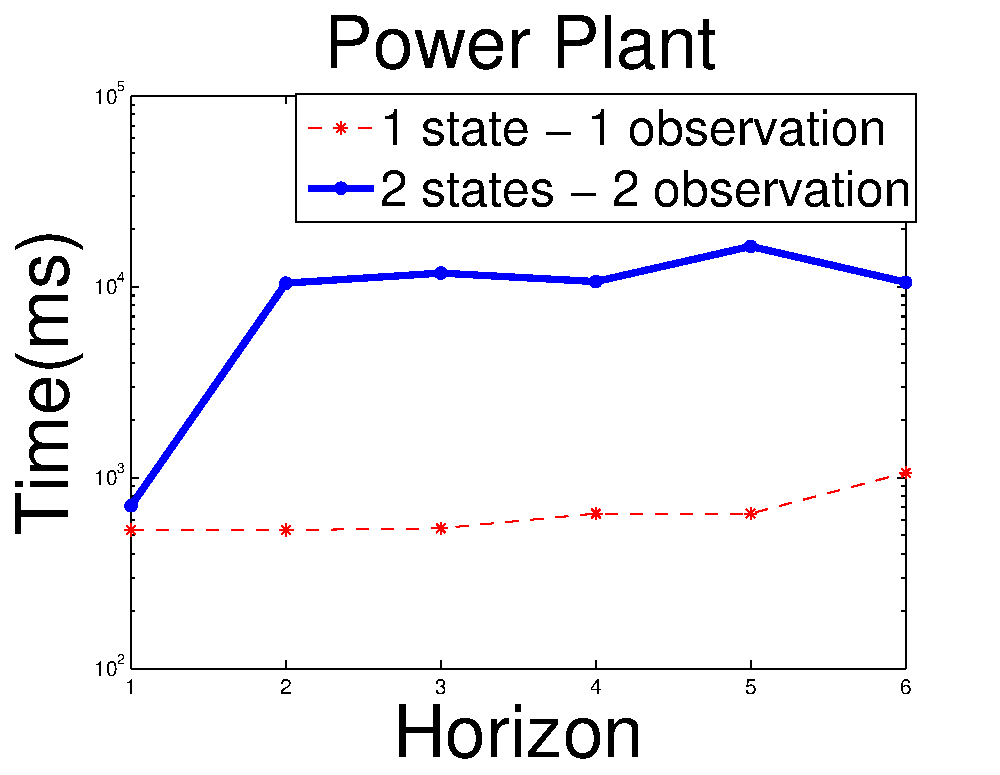
\includegraphics[width=0.3\textwidth]{pics/time2.pdf}
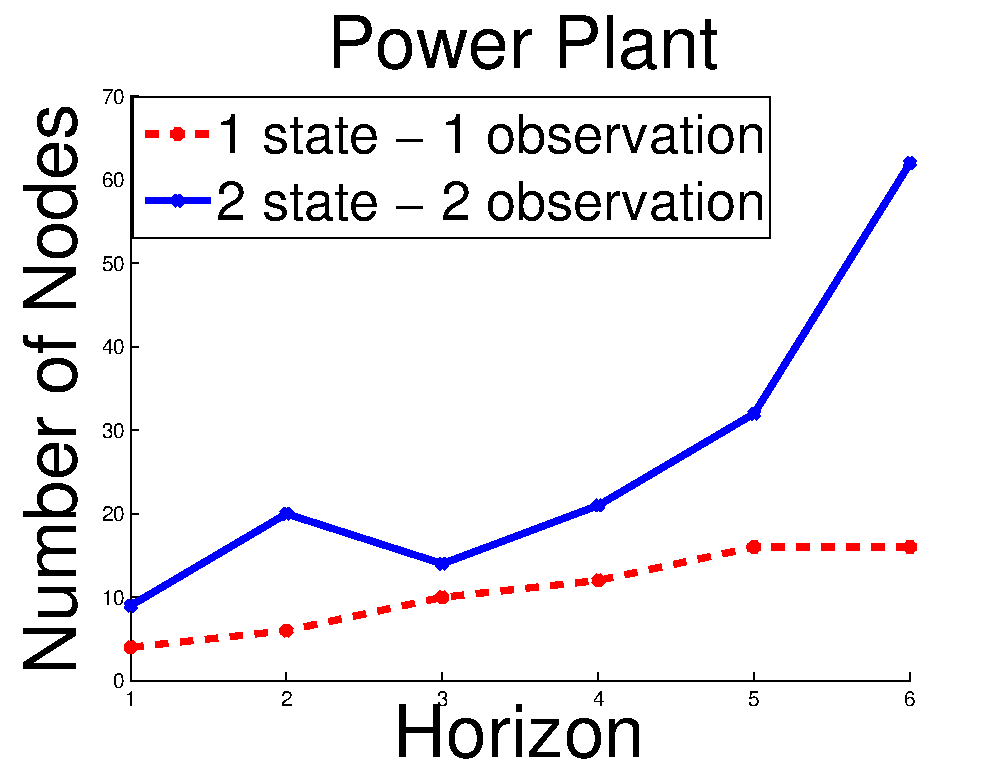
\includegraphics[width=0.3\textwidth]{pics/nodes2.pdf}
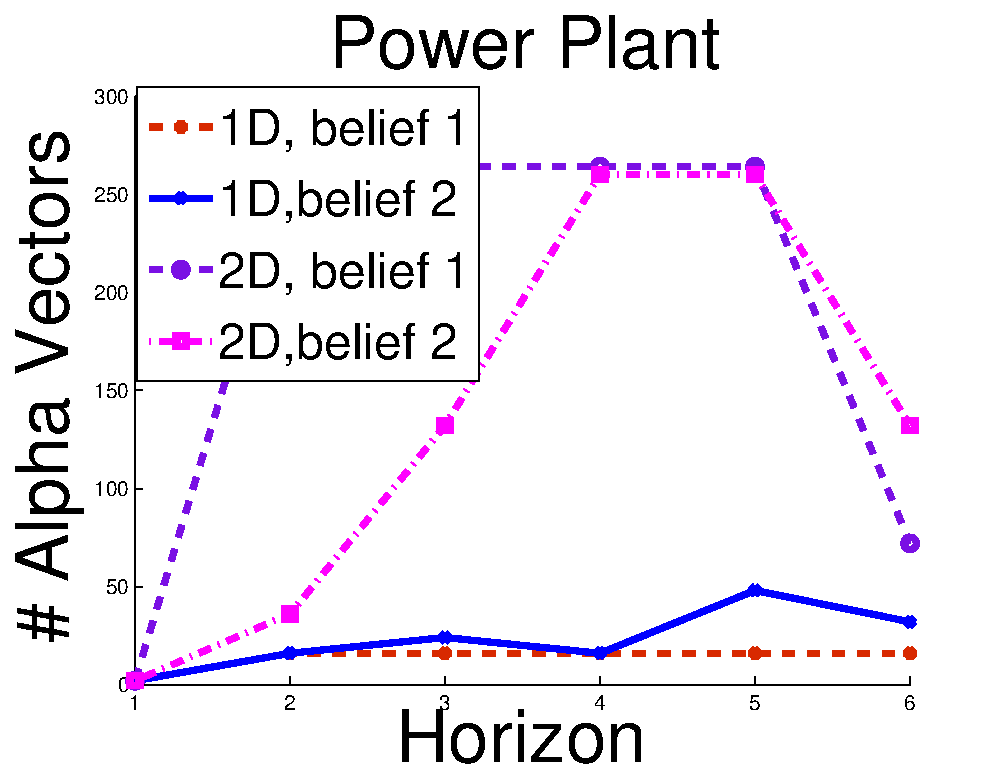
\includegraphics[width=0.3\textwidth]{pics/alpha-vectors2.pdf}
\vspace{-3mm}
\caption{\footnotesize 
{\it (left)} Space vs Horizon; 
{\it (middle)} Time vs Horizon; 
{\it (right)} Number of $\alpha$-vectors vs Horizon.
}
\label{fig:timeSpace}
\vspace{-4mm}
\end{figure*}
%%%%%%%%%%%%%%%%%%%%%%%%%%%%%%%%%%%%%%%%%%%%%%%%%%%%%%%%%%%%%%%%%%%%%%%%%% 

{\bf \textsc{2D-Power Plant}:} We consider the more complex model of the power plant similar to \cite{steam2} where the pressure inside the water tank must be controlled to avoid mixing water into the steam or explosion of the tank. We model the pressure variable $p$ as a partially observable variable from the observation readings of the pressure valve $po$. The two actions of increase and decrease are defined based on the change in both the temperature and the pressure. For the increase action the transition functions and the reward function is defined as below: 
{\footnotesize
\begin{align}
P(p_s'|\vec{p_s},a)&= \delta\left[ p_s' - 
\begin{cases}
 (p+10> 20) &: 20 \\ 
\neq (p+10> 20) &: p_s + 10 \\
\end{cases}
\right]\nonumber
\hspace{5mm} 
P(t_s'|\vec{t_s},a)= \delta\left[ t_s' -  t_s +10 \right]\nonumber
\\
R(t_s,p_s,a) &= 
\begin{cases}
(5 \leq p_s \leq 15)\wedge (95 \leq t_s \leq 105)&:50\\
(5 \leq p_s \leq 15)\wedge (t_s \leq 95)&: -1\\
(5 \leq p_s \leq 15)\wedge (t_s \geq 95)&: -3\\				
(p_s \leq 5) &: -3\\						
(p_s \geq 15) &: -5\\ 
\end{cases}\nonumber
\end{align}
}
There is a high reward for staying withing the safe temperature and pressure range since it produces power, else depending on how safe it is to have values higher or lower than the safe range, penalty is defined.
As for the decrease action, the transition functions reduce the temperature by 5 units and the pressure by 10 units as long as the pressure stays above zero. For the reward function, we assume that there is always a small penalty for decreasing the values because power can not be generated. 

For the observation model we consider two continuous uniform distributions such as the following:  
{\footnotesize
\begin{align}
P(t_o|t_s') = 
\begin{cases}
 (t_o>t_s + 80) \wedge (t_o<t_s+ 105) &: 0.4 \\
 \neg( (t_o>t_s + 80) \wedge (t_o<t_s+ 105)) &: 0 \\
\end{cases}\nonumber
\hspace{0mm} 
P(p_o|p_s') = 
\begin{cases}
 (p_o>p_s) \wedge (p_o<p_s+10) &: 0.1 \\
 \neg( (p_o>p_s) \wedge (p_o<p_s+10)) &: 0 \\
\end{cases}\nonumber
\end{align}
}
We define two rectangular uniform beliefs around the regions of rewarding, so that one needs to increase the values while the other should decrease them: $b_1: U[t_s;90,100]*U[p_s;0,10]$ and $b_2: U[t_s;90,130]*U[p_s;10,30]$
%\begin{align}
%b_1 = 
%\begin{cases}
%(p_o>p_s) \wedge (p_o<p_s+10) \wedge (t_o>t_s+ 90) \wedge (t_o<t_s+ 100)&: 0.01 \\
% \neg( (p_o>p_s) \wedge (p_o<p_s+10) \wedge (t_o>t_s+ 90) \wedge (t_o<t_s+ 100)) &: 0 \\
%\end{cases}\nonumber
%\end{align}
%\begin{align}
%b_2 = 
%\begin{cases}
%(p_o>p_s +10) \wedge (p_o<p_s+30) \wedge (t_o>t_s+ 90) \wedge (t_o<t_s+ 130)&: 0.00125 \\
% \neg((p_o>p_s +10) \wedge (p_o<p_s+30) \wedge (t_o>t_s+ 90) \wedge (t_o<t_s+ 130)) &: 0 
%\end{cases}\nonumber
%\end{align}
% I can draw this and the 1D belief
In Figure ~\ref{fig:timeSpace}, a time and space analysis of
the two versions of \textsc{Power Plant} have been performed for up to 6 horizons. Comparing the two problem sizes demonstrates the effect of the number of state-observation variables in our algorithm. As the algorithm progresses, the time required to compute the probability of the partitions and finding the maximum value function increases for both problem sizes and significantly more for the 2D version. The stability in time is due to the fact that each stage almost takes the same time since it has converged quickly.%???
Increase in the problem size, increases the partition numbers on the observation space and this produces more $\alpha$-vectors which also effects the space required to perform the algorithm. The number of vectors stays the same for most horizons and they drop after convergence in the 2D problem instance. The number of nodes in each iteration increases as more space is required to perform higher iterations. This shows that although the 2D instance takes more time and space than the 1D instance, it still converges within reasonable resources.

In Figure ~\ref{fig:3D}  we present plots of the value function for different iterations of the 2D problem instance. Each plot demonstrates the value as a function of the pressure and temperature. Starting with the first iteration, the value is highest for the reward range ($5<p<15 \wedge 95<t<105$) and -1 or less for other places. In the fifth iteration, the value function has partitioned into more pieces, showing how higher temperatures can increase the value without considering the effect of the pressure. In the last plot, horizon 6 has better tuned the value function so that higher temperatures and pressures increase the value function and also within the reward range, finer grain partitions have been formed. Also note that the policy depends on the initial belief and for these plots they were based on $b_1$ which was lower than the reward range. The first action would then mean it has performed an increase while the other iterations decrease and increase respectively.  
%%%%%%%%%%%%%%%%%%%%%%%%%%%%%%%%%%%%%%%%%%%%%%%%%%%%%%%%%%%%%%%%%%%%%%%%%%
% policy2, v2plot.pdf, v9plot
% annotation?
\begin{figure*}[tbp!]
\vspace{-2mm}
\centering
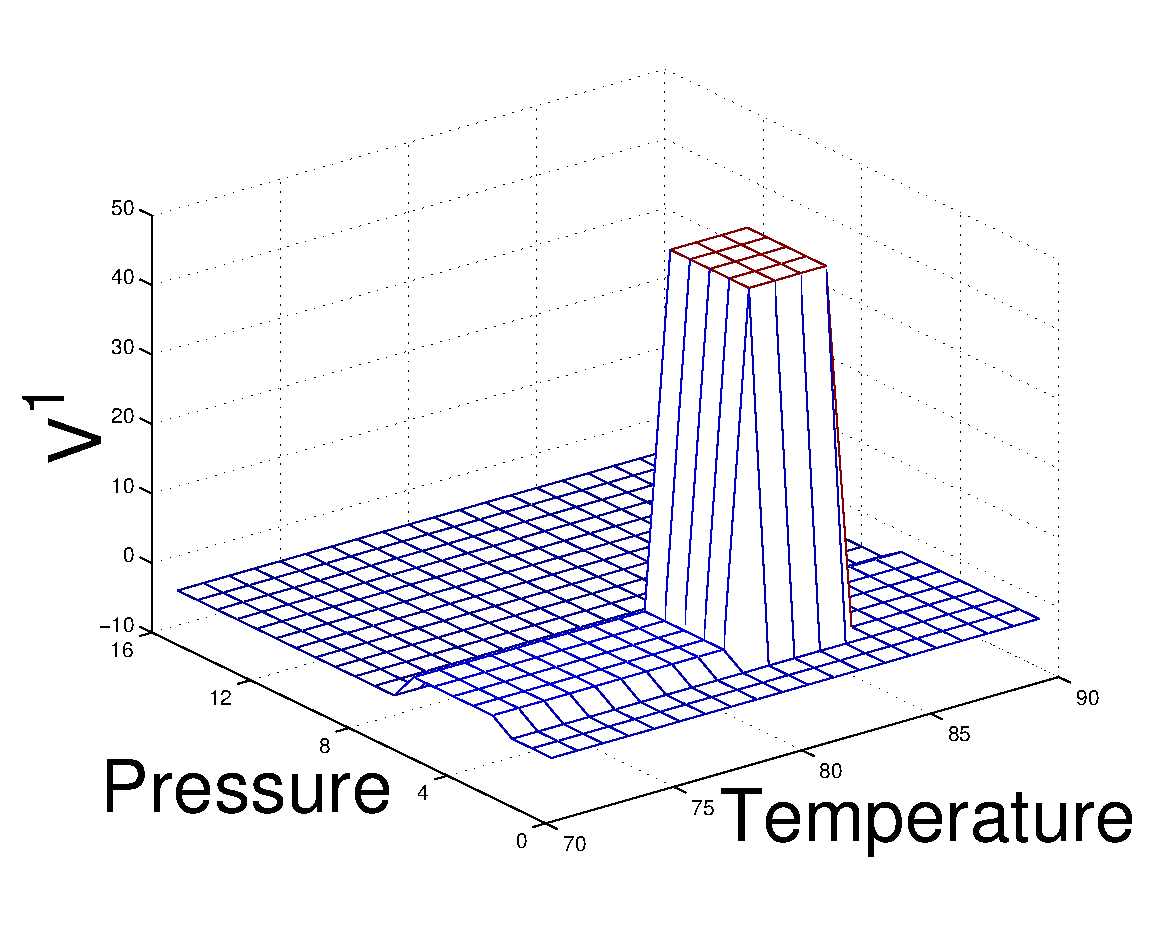
\includegraphics[width=0.31\textwidth]{pics/2d1.pdf}
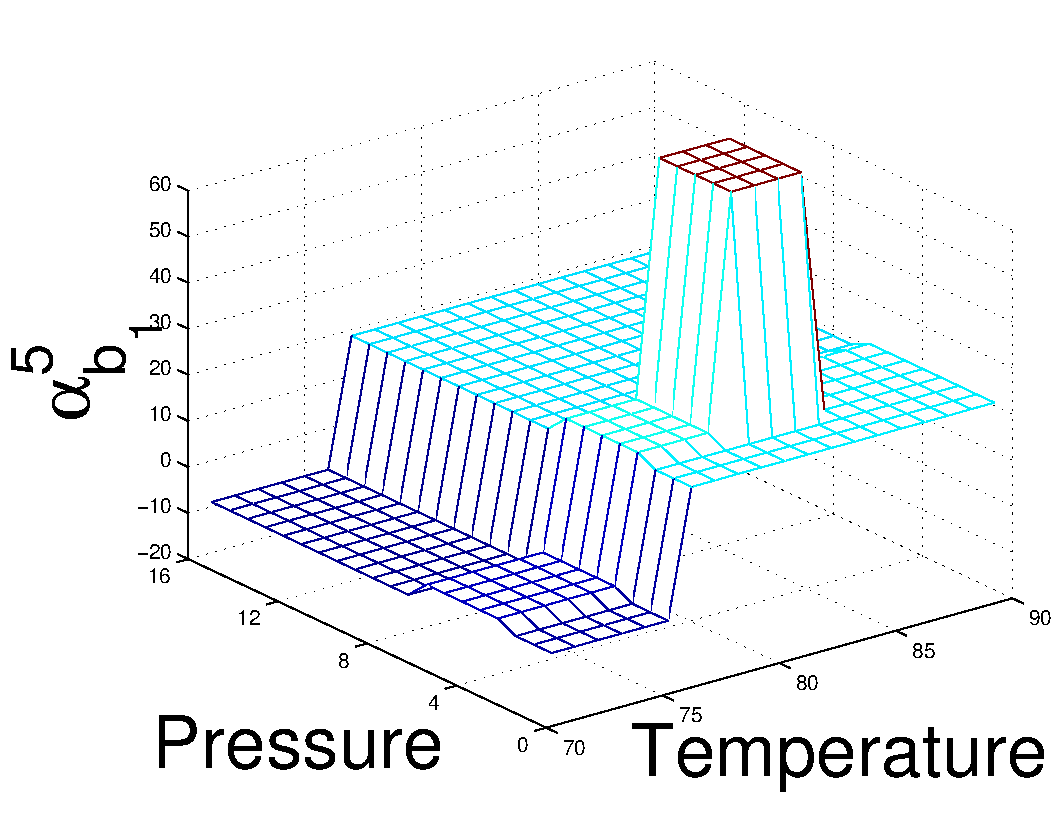
\includegraphics[width=0.31\textwidth]{pics/2d9.pdf}
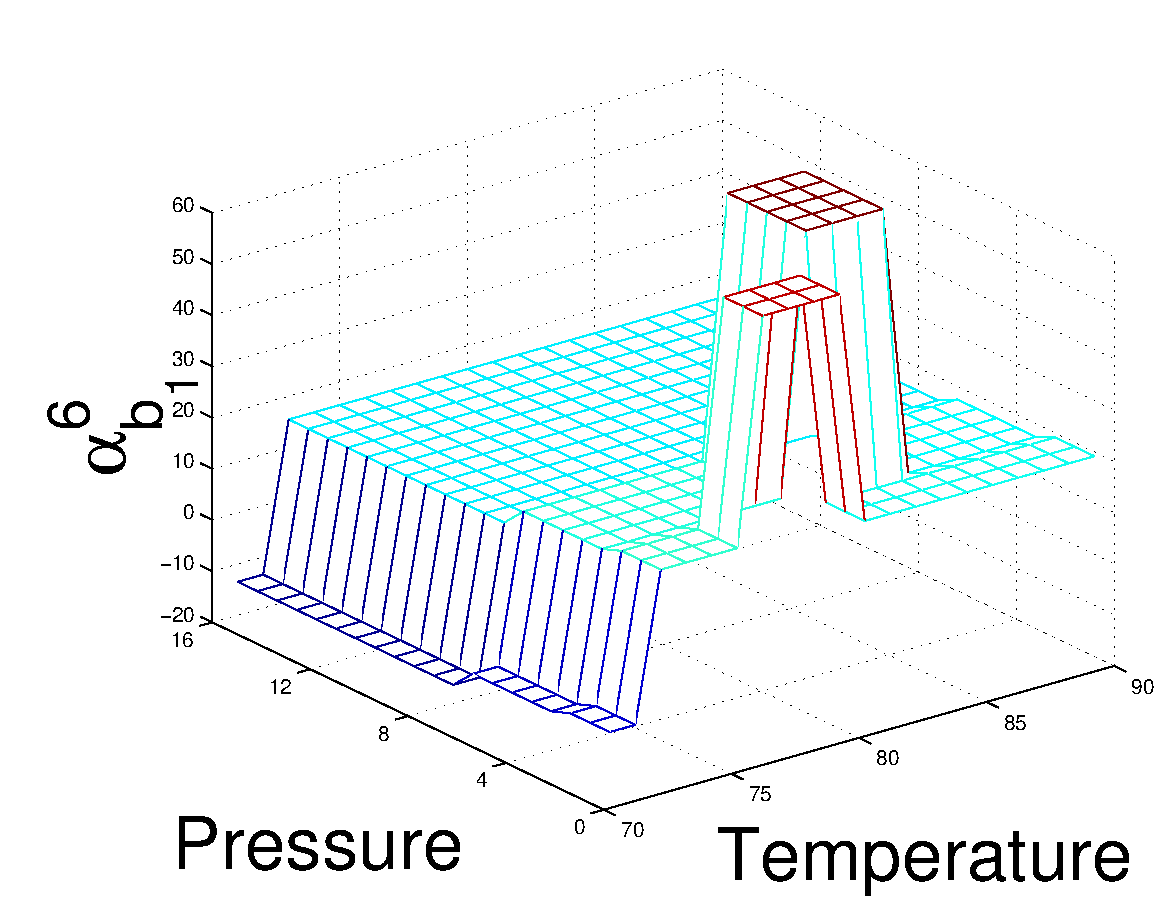
\includegraphics[width=0.31\textwidth]{pics/2d111.pdf}
\vspace{-3mm}
\caption{\footnotesize 
{\it (left)} Value function for first iteration; 
{\it (middle)} $V^5(p,t)$; 
{\it (right)} $V^6(p,t)$.
}
\label{fig:3D}
\vspace{-4mm}
\end{figure*}
%%%%%%%%%%%%%%%%%%%%%%%%%%%%%%%%%%%%%%%%%%%%%%%%%%%%%%%%%%%%%%%%%%%%%%%%%% 

\section{Related Work and Conclusion} 
This work has used the concept of continuous states and the SDP solution to MDPs from ~\cite{sanner_uai11} and continuous observations from the work of \cite{pascalPomdp}. It is exclusive in the sense that it brings together the continuous state and observation POMDPs using a symbolic approach. 
In many applications of the POMDP framework, the state and observation space have been considered as discrete values such as ~\cite{steam2} here we avoid this general simplification and work with the real values from sensors.
%sampling, monte carlo, particle filter, gaussians, perseus, pergeus

There has been prior work on approximate solutions to POMDPs with large or continuous state spaces ~\cite{Thrun99h}, ~\cite{Perseus} and some has been extended to the continuous observation setting using methods such as sampling ~\cite{PerseusObs}.
In most approximate continuous state POMDP work, continuous or large discrete actions has been used. Thus we can extend the current work using \cite{zamaniAAAI} to contain continuous actions and provide exact or approximate solutions. 

%\section{Conclusion}
We presented the first exact solution to continuous states and observations in a DC-POMDP framework. Transitions and reward functions are defined as piecewise linear functions of the continuous states. Continuous observations require definition of explicit partitions based on the observation model and the belief state of the agent. The key contribution is to define the partitions on the observation space and derive the related probabilities using symbolic integration and maximization. We extend the application to more than one state-observation setting and present the results.  
 
%\subsubsection*{References} 
\bibliography{dcpomdp}
\bibliographystyle{plain}

\end{document}
